\documentclass[]{article}
\usepackage[utf8]{inputenc}
\usepackage[ngerman]{babel}
\usepackage{textcomp}
\usepackage{hyperref}
\usepackage{graphicx}
\usepackage{float}


\usepackage{listings}
\lstset{
	language=C++,
	tabsize=4,
	keepspaces,
	extendedchars=true,
	rulecolor=\color{black},
	basicstyle=\footnotesize,
	aboveskip=5pt,
	upquote=true,
	columns=fixed,
	showstringspaces=false,
	extendedchars=true,
	breaklines=true,
	frame=single,
	showtabs=true,
	showspaces=false,
	showstringspaces=false,
	basicstyle=\tiny,
	keywordstyle=\color{blue}
}

%opening
\title{First steps}
\author{Wombacher Sascha}

\begin{document}
\maketitle


\section{Introduction}

This small guide will help you install and run all provided examples and provide some info about how to add your own project(s).

\mbox{} \\
\textbf{Getting started:}
\begin{itemize}
	\item Introduction for Windows users (section \ref{Windows})
	\item Introduction for \space macOS \space \space users (section \ref{Mac})
	\item Introduction for \space \space Linux \space \space \space users (section \ref{Linux})
\end{itemize}

\mbox{} \\
\textbf{Available documentation} (located in \textit{$<$ProjectDirectory$>$/Documentation}):
\begin{itemize}
\item HTML (recommended)
\item PDF
\end{itemize}

\mbox{}\\
\textbf{Other:}
\begin{itemize}
	\item Fist of all good luck and have fun :)
	\item If you have any feedback I'd love to hear any suggestions :)
\end{itemize}


\section{General}
This library uses some third Party libraries and tools:
\begin{itemize}
	\item GLM (GL mathematics for vector and matrix operations)
	\item OpenCV (ComputerVision library for 2D graphics)
	\item Glut/Freeglut (3D, currently only OpenGL 1.x is used)
	\item BigInt (Lib for very long int values, C\# equivalent BigInt)
	\item Swig (tool for generating a Python to this library)
\end{itemize}

\newpage
\section{Windows}\label{Windows}

Insatllation:
\begin{itemize}
	\item Install VisualStudio 2017 or VisualStudio 2017 Redistributable (64-Bit):
	\begin{itemize}
		\item Provided: VC\_redis.x64.exe
		\item Link:\\ \url{https://www.visualstudio.com/downloads/}
	\end{itemize}
	
	\mbox{}\\
	\item 
	Install Python (3.6.5 tested):
	\begin{itemize}
		\item Provided: python-3.6.5-amd64.exe   
		\item Link, 64-Bit version required!:\\ \url{https://www.python.org/downloads/release/python-365/} 
		\item \textbf{IMPORTANT:\\You have to add Python to your \textit{PATH}-Variables}
		\begin{figure}[H]
			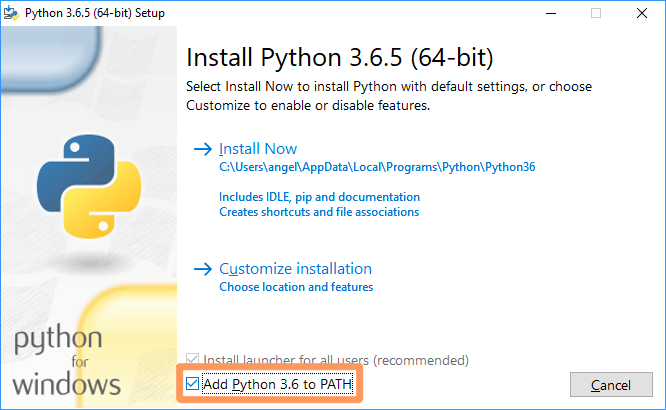
\includegraphics[width=\linewidth]{pythonPathVariable.png}
		\end{figure}
	\end{itemize}

	\item Test your installation
	
\end{itemize}


\newpage
\section{Mac}\label{Mac}

Installation:
\begin{itemize}
	\item To install dependencies run: \textbf{'mac\_installDependencies.sh'}
	\item To test your installation:
	\begin{itemize}
		\item Open a console
		\item Change directory into \textit{$<$ProjectDirectory$>$/PythonSolutions}
		\item Start the example file by running: \textbf{'python computerGeometry\_example.py'}
	\end{itemize}
\end{itemize}

\newpage
\section{Linux}\label{Linux}

\mbox{}\\
Installation:
\begin{itemize}
	\item To install dependencies run: \textbf{'linux\_installDependencies.sh'}
	\item To test your installation:
	\begin{itemize}
		\item Open a console
		\item Change directory into \textit{$<$ProjectDirectory$>$/PythonSolutions}
		\item Start the example file by running: \textbf{'python computerGeometry\_example.py'}
	\end{itemize}
\end{itemize}

\end{document}
